\pagebreak
\section{SOP: Setting up LimeSurvey for compatibility with ALIIAS}
\label{section:ls_setup}

\subsection*{General information about LimeSurvey}
\addcontentsline{toc}{subsubsection}{General information about LimeSurvey}

\begin{wrapfigure}{r}{0.5\textwidth}
\centering
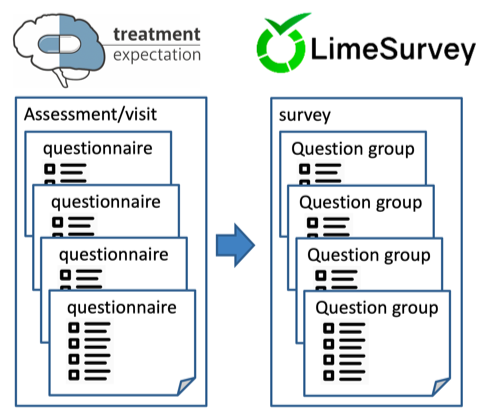
\includegraphics{docs/fig/ls_conventions.png}
\caption{LimeSurvey's terminology.}
\label{fig:ls_conventions}
\end{wrapfigure}

LimeSurvey (\href{www.limesurvey.org}{\color{pniblue} www.limesurvey.org}) is a free and open source on-line statistical survey web application.
In LimeSurvey, a series of questions, which are supposed to be filled-in by the same person, in one session; is called a \emph{survey} ("Umfrage", Fig. \ref{fig:ls_conventions}).
In SFB289, multiple assessment points or visits within one study will be represented by multiple surveys.
A survey typically consists of many questionnaires (“Fragebögen”), which are called “question groups” in LimeSurvey.
LimeSurvey provides the opportunity to limit survey access to those participants only, who were previously registered to a so-called participant table (“Teilnehmertabelle”) of the survey by the researcher. In SFB289, ALIIAS will generate pseudonyms for participants and – after the proper setup of LS – automatically register the participants (with their pseudonyms) to the surveys specified by the researcher. Moreover, the link (URL) for these surveys can also be obtained from ALIIAS. The following steps explain how to set up LimeSurvey for compatibility with ALIIAS.

\par\noindent\rule{\textwidth\color{pniblue}}{0.4pt}
\subsection*{Step 1. Log in to LimeSurvey.}
\addcontentsline{toc}{subsubsection}{LimeSurvey login}
The URL for the CRC-wise LimeSurvey server is:

\hyperref[https://sfb289.survey.uni-due.de/index.php/admin/authentication/sa/login]{https://sfb289.survey.uni-due.de/index.php/admin/authentication/sa/login}

Log in credentials will be sent out individually. 


\small\setlength\fboxsep{5pt}\setlength\fboxrule{1pt}
\fcolorbox{pniblue}{pniblue!5}{\begin{minipage}{0.9\textwidth}
In case of trouble during log in, see point \ref{faq:ls_login} in section \ref{section:faq} ("Troubleshooting").
\end{minipage}}

\large
\par\noindent\rule{\textwidth\color{pniblue}}{0.4pt}
\subsection*{ Step 2. Creating a new SFB289-survey.}
\addcontentsline{toc}{subsubsection}{Create survey}
The single projects in SFB289 can have multiple surveys, e.g. one survey for each measurement time point (“visit”). For studies in which the researcher or study doctor is also supposed to fill in a questionnaire/checklist, multiple surveys for each visit should be used (see step 2.3).

When creating a new survey, we have access to the standard questionnaire battery of SFB289. To include it, new surveys must be created by copying the survey \\ “SFB289\_standard\_questionnaire\_battery” as many times as needed. 

\par\noindent\rule{\textwidth\color{pniblue}}{0.4pt}
\subsubsection*{2.1. Choose “Kopieren Sie eine Umfrage” on the home screen.}
\begin{figure}[H]
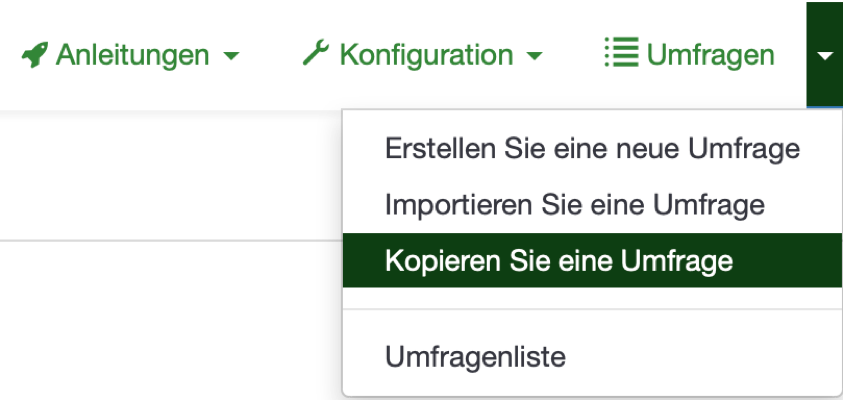
\includegraphics[width=0.5\textwidth]{docs/fig/ls_sop2.1.png}
\end{figure}

\par\noindent\rule{\textwidth\color{pniblue}}{0.4pt}
\subsubsection*{2.2 Select the “Kopieren” tab, select the survey called “SFB289\_standard\_questionnaire\_battery” to copy from. }
\begin{figure}[H]
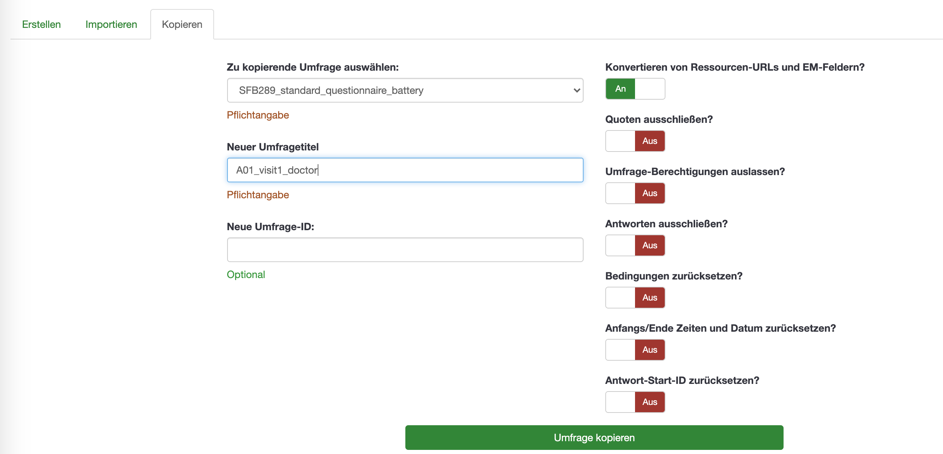
\includegraphics[width=1.0\textwidth]{docs/fig/ls_sop2.2.png}
\end{figure}

\par\noindent\rule{\textwidth\color{pniblue}}{0.4pt}
\subsubsection*{2.3 Give the new survey a name according to the following rule:} <project>\_<study>\_<measurement>\_<target>

\subsubsection*{Explanation:}
\begin{itemize}
    \item <project>: the name of the single project within the SFB. Must consist of an uppercase “A” letter and a two-digit number (A01, A02, …, A16). Our pseudonymization software (called ALIIAS) uses this part of the name to restrict visibility of surveys.
    \item <study>: an arbitrary identifier to distinguish studies if multiple studies are performed within one project. (e.g. study1, follow-up, etc.). Can be omitted if only one study is performed. 
    \item <measurement>: a name for measurement time point (e.g. baseline, visit1, day1, pre, post, etc). Can be omitted if the study involves only one measurement time point.
    \item <target>: the “role” of the person who fills in the survey. (e.g. participant, doctor, interviewer, etc). Can be omitted if all surveys are filled in by the participants.
\end{itemize}

Separator must be underscore (\_). Refer to Table \ref{tab:example_names} for some valid examples for survey names. Click on “Umfrage kopieren” to create the new survey.
\begin{table}[h]
 \caption{Example survey names, compatible with ALIIAS.}
  \centering
  \begin{tabular}{ll}
    \toprule
    Survey names      & Explanation      \\
    \midrule
    \midrule
    A01            & a hypothetical A01 project consisting of a single survey only                 \\
    \midrule
    A02\_visit1           & a hypothetical A02 project, having two visits \\
    A02\_visit2      & \\
    \midrule
    A03\_study1           & a hypothetical A03 project,               \\
    A03\_study2\_visit1          &  having two studies and two visits in the second study              \\
    A03\_study1\_visit2           &                \\
    \midrule
    A04\_visit1\_participant      &   a hypothetical A04 project,             \\
    A04\_visit1\_doctor           &   having separate surveys for the participant and the study doctor           \\
    \bottomrule
  \end{tabular}
  \label{tab:example_names}
\end{table}

\par\noindent\rule{\textwidth\color{pniblue}}{0.4pt}
\subsection*{Step 3. Edit the new survey as needed. }
\addcontentsline{toc}{subsubsection}{Customize survey}

\begin{wrapfigure}{r}{0.5\textwidth}
\centering
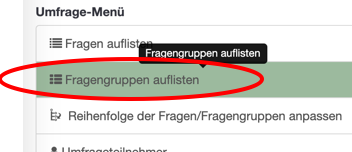
\includegraphics{docs/fig/ls_sop3.png}
\end{wrapfigure}

Questionnaires within the survey are represented by question groups in LS.
Navigate to the page of the new survey (“Umfragen” -> “Umfragenliste” -> select previously created project) and choose the “Fragengruppen auflisten” menupoint (left-sided menu) in the “Umfrage-Menü”.

\par\noindent\rule{\textwidth\color{pniblue}}{0.4pt}
\subsubsection*{3.1 Remove unnecessary question groups (if any).}
\begin{wrapfigure}{r}{0.5\textwidth}
\centering

\includegraphics{docs/fig/ls_sop3.1.png}
\end{wrapfigure}

Surveys can be edited with the following control buttons: 
Remove any questionnaires ("question groups") that are not needed for the given survey (refer to the study proposal).

\par\noindent\rule{\textwidth\color{pniblue}}{0.4pt}
\subsubsection*{3.2 Add any additional surveys that are needed for the survey, according to the study proposal.}

\begin{wrapfigure}{r}{0.5\textwidth}
\centering

\includegraphics{docs/fig/ls_sop3.2.png}
\end{wrapfigure}

Additional surveys can be either added manually or imported.
Before starting to implement extra (study-specific) surveys (via “Neue Gruppe hinzufügen”), please contact Katharina Schmidt (\href{mailto:katharina.schmidt@uk-essen.de}{katharina.schmidt@uk-essen.de}),  Julian Kleine-Borgmann (\href{mailto:julian.kleine-borgmann@uk-essen.de}{julian.kleine-borgmann@uk-essen.de}) and Tamas Spisak (\href{mailto:tamas.spisak@uk-essen.de}{tamas.spisak@uk-essen.de}). The needed questionnaire might have already been implemented and can be imported with the “Eine Gruppe importieren” button.

\par\noindent\rule{\textwidth\color{pniblue}}{0.4pt}
\subsection*{Step 4. Activate the new survey}
\addcontentsline{toc}{subsubsection}{Activate survey}

\begin{wrapfigure}{r}{0.5\textwidth}
\centering

\includegraphics{docs/fig/ls_sop4_home.png}

\includegraphics{docs/fig/ls_sop4_button.png}
\end{wrapfigure}

Navigate to the main page of the survey by clicking the “home” button on the top left. Click the “Diese Umfrage aktivieren” button. At the next page, accept the default settings and click “Speichern \& Umfrage aktivieren”:

\begin{figure}[H]
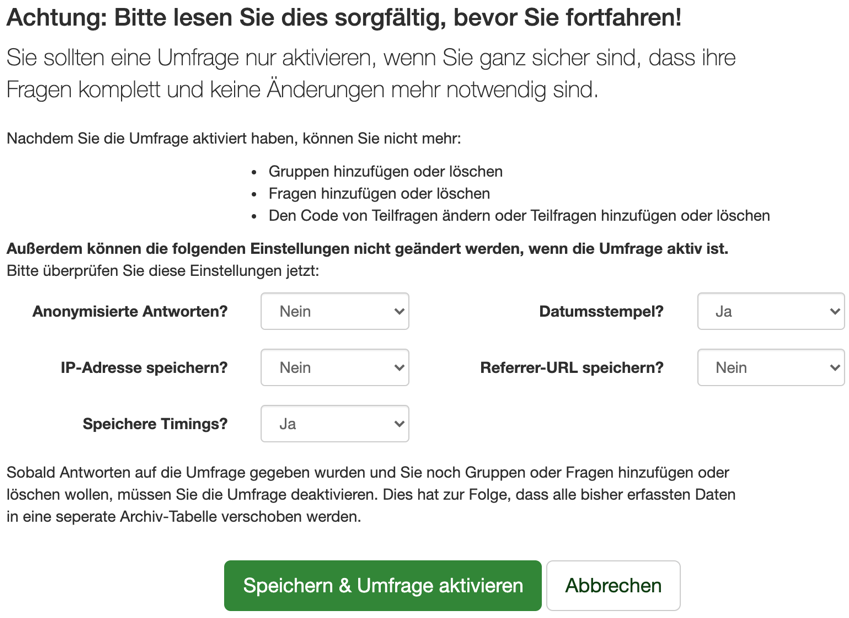
\includegraphics[width=0.7\textwidth]{docs/fig/ls_sop_4.png}
\end{figure}

\par\noindent\rule{\textwidth\color{pniblue}}{0.4pt}
At the next page switch to closed mode (“zum geschlossenen Modus umschalten”) so that the questionnaire won’t be accessible without invitation:

\begin{figure}[H]
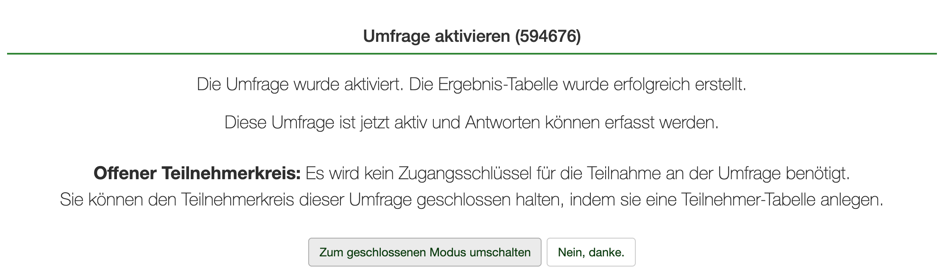
\includegraphics[width=0.7\textwidth]{docs/fig/ls_sop4.1.png}
\end{figure}

\par\noindent\rule{\textwidth\color{pniblue}}{0.4pt}
At the next page, initialize a participant table when prompted to do so. Only those participants can be invited to the survey who were previously registered in this survey-specific participant table. In SFB289, the participant table will be manipulated (e.g. adding new participant or generating access tokens and survey links) not directly in LS, but through the interfaces of ALIIAS, to ensure anonymity and consistency in LS (more details in the ALIIAS manual).

\begin{figure}[H]
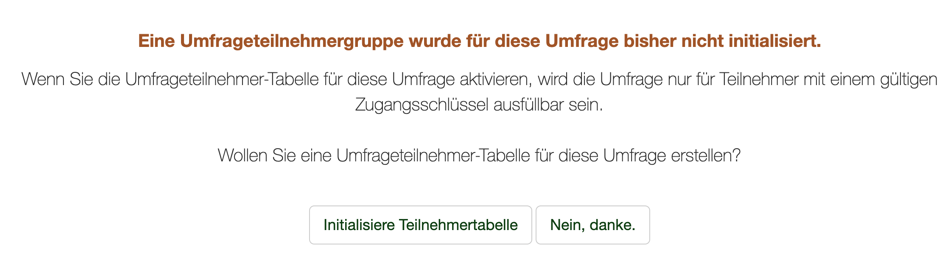
\includegraphics[width=0.7\textwidth]{docs/fig/ls_sop4.2.png}
\end{figure}

\par\noindent\rule{\textwidth\color{pniblue}}{0.4pt}
After clicking on “Weiter”, setting up the survey for ALIIAS compatibility is finished and the user can log out of LimeSurvey (by clicking in the user name in the top right corner and selecting 'Abmeldung').

\par\noindent\rule{\textwidth\color{pniblue}}{0.4pt}
\subsection*{Information about further use of the surveys}
\addcontentsline{toc}{subsubsection}{Using surveys and exporting results}
After these steps, the new surveys are ready to be used together with the pseudonymization software ALIIAS. Participants added to this survey can always be listed by clicking the button “Umfrageteilnehmer” on the main page of the questionnaire and then the “Zeige Teilnehmer” Button (top survey-menubar). 

\begin{figure}[H]
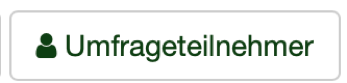
\includegraphics[width=0.2\textwidth]{docs/fig/ls_sop4_umfrageteilnehmer.png}
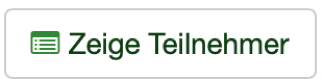
\includegraphics[width=0.2\textwidth]{docs/fig/ls_sop4_zeige_teilnehmer.png}
\end{figure}

\small\setlength\fboxsep{5pt}\setlength\fboxrule{1pt}
\fcolorbox{pniblue}{pniblue!5}{\begin{minipage}{0.9\textwidth}
The surveys only have to be set up in LS once, at project start. After this, the preferred way of interacting with LS is the interface provided by the pseudonymization software ALIIAS. LS should only be used for purposes of double-checking and manual corrections, if required.
\end{minipage}}

\large

\subsubsection*{Adding and inviting a new participant to a survey}
ALIIAS provides all interfaces to LS that are typically required during experimental studies. For instance, when generating a new pseudonym, ALIIAS provides the opportunity to automatically register the participant with the new pseudonym in LS to the selected surveys. ALIIAS restricts the visibility of surveys, so that members of a single project can only see and manipulate their own surveys. With ALIIAS, it is easy to find out if a participant has already been registered to any of the surveys. Through ALIIAS, we can obtain the participant-related “invitation” links to any surveys. These links can be simply opened in the browser on any computer or sent out to the participant in an e-mail.


\small\setlength\fboxsep{5pt}\setlength\fboxrule{1pt}
\fcolorbox{pniblue}{pniblue!5}{\begin{minipage}{0.9\textwidth}
For detailed description of the process, refer to the SOP in the next section (section \ref{section:sop_ls})
\end{minipage}}

\large

\subsubsection*{Saving questionnaire data}
For legal reasons (and to defend against discrimination attacks), the LS database will be regularly (each night at 2am) “flushed”, that means, questionnaire data (responses) will be automatically moved to a safe local storage. Therefore, the export of questionnaire data is not possible with the export function of LS. Instead, the latest version of the database will be available on a private Sciebo link for the single projects, as a csv file and excel table. This database will be automatically updated each night.



